\documentclass{foi}
\usepackage[utf8]{inputenc}
\usepackage{lipsum}

\vrstaRada{\projekt} % \diplomski
\title{Rad s XML u Javi}

\author{Hrvoje Lesar}
\spolStudenta{\musko} % \zensko ili \musko

\mentor{Sandro Gerić}
\spolMentora{\musko} % \zensko ili \musko
\godina{2023}
\mjesec{Svibanj}
\date{2023}
\indeks{0016133479}
\smjer{Organizacija poslovnih sustava}
\titulaProfesora{Izv. prof. dr. sc.}

\begin{document}

\maketitle

\tableofcontents

\pagestyle{plain}

\chapter{Uvod}
Kroz rad će se biti objašnjen XML; kakav je to format, biti će definirana pravila koja
se moraju poštivati kod pisanja XML-a, struktura XML dokumenta. Nadalje ćemo pregledati
kako se XML koristi u programskom jeziku Java, te pokazati kako ga na više načina
parsirati i provjeravati da dokument odgovara priloženoj XSD shemi.

Izvan ovog dokumenta projekt je strukturiran u dvije cjeline; Jedna cjelina je
dokumentacija tj. LaTeX dokument i skripte kojima se može generirati ovaj pdf.
Drugi dio je izvorni kod. U direktoriju s izvornim kodom je priložena datoteka
README.md u kojoj je dokumentirano kako se može kompajlirati i pokrenuti izrađeni
program. Program je jednostavna konzolna aplikacija koja ispisuje vremensku prognozu
iz priloženih XML datoteka \cite{dhmz}. Zbog lakšeg pokretanja programa postavljena je
izvršna datoteka u direktorij s izvornim kodom, da bi se izbjegla potreba za kompalacijom koda.


\chapter{XML}
XML je standard za označavanje dokumenata koji podržava W3C organizacija.
Kratica XML stoji za Extensible Markup Language. Kroz XML se definira generička
sintaksa korištena za označavanje podataka jednostavnim, za ljude čitljivim oznakama \cite{xml_in_a_nutshell}.
Ovakav format dokumenta omogućuje visoku razinu kostumizacije načina definiranja
i prikaza podataka. Neki od primjera gdje se koristi su vektorska grafika,
elektronička razmjena podataka, serijalizacija objekata (pretvaranje Java objekta u XML dokument),
poziva udaljenih procedura.

\section{Struktura}
Podatci u XML dokumentu su zapisani kao tekst. Podatci su okruženi tekstualnim oznakama
koje opisuju podatak. Osnovna jedinica podatka i oznake naziva se element. U nastavku će
biti definirane ostale vrste čvorova dostupnih u XML sintaksi. XML specifikacija definira
točnu sintaksu koja se u dokumentu mora poštivati, definira kako su elementi orkuženi
oznakama (tagovima), kako izgleda tag, koji nazivi tagova su prihvatljivi, gdje se
atributi nalaze i njihovu sintaksu.

\begin{lstlisting}[caption={Vrste čvorova}]
<?xml version="1.0" encoding="UTF-8"?>
<Hrvatska>
    <!-- Prognoza za datum 20.05.2023. -->
    <DatumTermin>
        <Datum>20.05.2023</Datum>
        <Termin>20</Termin>
    </DatumTermin>
    <Grad autom="0">
        <GradIme>Varaždin</GradIme>
        <Lat> 46.28</Lat>
        <Lon> 16.36</Lon>
        <Podatci>
            <Temp> 19.7</Temp>
            <Vlaga>75</Vlaga>
            <Tlak>1015.2</Tlak>
            <TlakTend>-</TlakTend>
            <VjetarSmjer>NE</VjetarSmjer>
            <VjetarBrzina> 3.5</VjetarBrzina>
            <Vrijeme>pretežno oblačno</Vrijeme>
            <VrijemeZnak>4</VrijemeZnak>
        </Podatci>
    </Grad>
</Hrvatska>
\end{lstlisting}

U isječku je prikazan jedan XML dokument. Dokument prikazuje prognozu vremena
na određeni dan. Kroz dokument možemo vidjeti različite vrste čvorova koje XML
sintaksa podržava tj. možemo definirati 5 vrsta:
\begin{enumerate}
	\item Uputa za obradu (meta element) - u prvoj liniji definirani je meta element koji
	      opisuje dokument. Prikazani element definira verziju XML-a koju prikazuje dokument
	      i vrstu kodiranja teksta. Meta elementi se koriste za opis dokumenta i ne mogu imati
	      sadržavati druge elemente.
	\item Korijenski element - u primjeru je korijenski element prikazan tagom \texttt{Hrvatska}.
	      Pravilni XML dokument mora sadržavati točno jedan korijenski element u kojemu su sadržani
	      svi ostali elementi dokumenta.
	\item Element - XML element s nazivom, atributima i listom elemenata djece. Primjer
	      elementa može biti bilo koji od elemenata definiranih poslije korijenskog. Element
	      \texttt{Grad} je dobar primjer elementa koji sadrži više elemenata djece, sadrži
	      jedan atribut nazvan \texttt{autom} s vrijednošću \texttt{0}.
	\item Tekst - niz znakova između otvarajućeg i zatvarajućeg taga. \texttt{Varaždin} je
	      primjer teksta, vrijednosti koju sadrđi tag \texttt{GradIme}.
	\item Komentar - koristan za ostavljanje napomena ili komentara u dokumentu. Kod parsiranja
	      ovaj element se preskače. U primjeru se komentar nalazi u trećoj liniji, komentar ne može
	      sadržavati druge elemente, sadržaj komentara su podaci komentara.
\end{enumerate}

\section{Pravila}
Pravilno oblikovanje dokumenta je minimalni zahtjev za XML dokument \cite{w3c_rec}.
Dokument koji nije pravilno oblikovan nije XML dokument. Parseri ga ne mogu pročitati i
nije im dozvoljeno popravljati neispravan dokument, ne može pretpostaviti za koju
svrhu je autor namijenio dokument te ispraviti dokument, kao što je moguće kod HTML-a.
Kako bi XML dokument bio pravilno oblikovan mora sadržavati \cite{process_xml}:
\begin{itemize}
	\item točno jedan korijenski element,
	\item svi početni tagovi moraju imati završne tagove,
	\item vrijednosti u atributima moraju biti u navodnicima,
	\item sadržaj mora biti definiran unutar character seta,
	\item tagovi mogu biti ugniježđeni ali se ne smiju preklapati.
\end{itemize}

\chapter{XML u javi}
U ovom poglavlju ćemo proći kroz nekoliko načina učitavanja i parsiranja XML datoteke
u programskom jeziku Java. Prikazati kako su pristupi parsiranju različiti te koje su
prednosti i nedostaci kod korištenja određene vrste parsera.

\section{XSD}
XSD je kratica za XML Schema Definition. XSD se koristi za definiranje strukture XML
dokumenta, sama shema je pisana u XML-u.
Svi podaci koji se u java projektu učitavaju prvo se validiraju prema XSD zadanoj shemi.
U projektu su korišteni tri različiti XML dokumenti što znači da ujedno postoje i
tri različite XSD sheme.

\begin{lstlisting}[caption={Primjer XSD dokumenta za sedmodnevnu prognozu vremena}]
<xs:schema xmlns:xs="http://www.w3.org/2001/XMLSchema">

    <xs:complexType name="grad">
        <xs:sequence>
            <xs:element name="GradIme" type="xs:string" />
            <xs:element name="Tmax" type="xs:string" />
            <xs:element name="Tmin" type="xs:string" />
            <xs:element name="Tmin5" type="xs:string" />
            <xs:element name="Obor" type="xs:double" />
            <xs:element name="Snijeg" type="xs:string" />
            <xs:element name="VlagaMax" type="xs:integer" />
            <xs:element name="VlagaMin" type="xs:integer" />
            <xs:element name="Sunce" type="xs:string" />
            <xs:element name="Tna5Max" type="xs:string" />
            <xs:element name="Tna5Min" type="xs:string" />
            <xs:element name="Tna20Max" type="xs:string" />
            <xs:element name="Tna20Min" type="xs:string" />
        </xs:sequence>
    </xs:complexType>

    <xs:complexType name="podaci">
        <xs:sequence>
            <xs:element name="Grad" type="grad" minOccurs="0" maxOccurs="unbounded" />
        </xs:sequence>
    </xs:complexType>

    <xs:complexType name="agroMeteoroloskiPodaci">
        <xs:sequence>
            <xs:element name="Naslov" type="xs:string" />
            <xs:element name="Podaci" type="podaci" />
        </xs:sequence>
    </xs:complexType>

    <xs:element name="AgroMeteoroloskiPodaci" type="agroMeteoroloskiPodaci" />

</xs:schema>
\end{lstlisting}

Kroz priloženi dokument je definirana struktura XML dokumenta koji će sadržavati podatke
o sedmodnevnoj prognozi vremena. Shema definira jedan korijenski element koji ima prilagođeni tip podatka.
\texttt{AgroMeteoroloskiPodaci} je korijenski element koji mora biti prisutan u XML dokumentu
koji ova shema validira. Korijenski element mora se sastojati od dva druga elementa, a to su
\texttt{Naslov} i \texttt{Podaci}. \texttt{Naslov} je jednostavni element koji sadrži vrijednost
naslova, dok su \texttt{Podaci} element koji se sastoji od više podelemenata tipa \texttt{Grad}.

\begin{lstlisting}[language=java, caption={Klasa za validaciju XML datoteke prema XSD shemi}]
public class XSDValidator {
    public static void validiraj(File xmlDat, File xsdDat) throws SAXException, IOException {
        SchemaFactory schemaFactory = SchemaFactory.newInstance(XMLConstants.W3C_XML_SCHEMA_NS_URI);
        Schema schema = schemaFactory.newSchema(xsdDat);
        Validator validator = schema.newValidator();
        validator.validate(new StreamSource(xmlDat));
    }
}
\end{lstlisting}

Klasa sadrži jednu metodu koja kao ulaz prima XML datoteku i XSD datoteku.
U metodi se kreira nova instanca \texttt{SchemaFactory} koja kao arugment prima putanju
do sheme koja će se koristiti za validaciju XML dokumenta. U ovom slučaju se koristi
ugrađena konstana \texttt{XMLConstants$.$W3C\_XML\_SCHEMA\_NS\_URI} koja je zapravo
putanja na imenski prostor (namespace) XSD sheme koji definira pravila sheme.
Potom se kreira nova instanca sheme koja za ulazni argument uzima datoteku
sheme, poslijednje se kreira objekt validator kojemu se predaje XML datoteka koju
želimo validirati prema zadanoj shemi. U slučaju da nije moguće validirati ulaznu
datoteku validator postavlja iznimku i valja grešku kod validiranja dokumenta.

\section{SAX}
SAX je prva vrsta parsera koju ćemo pregledati. SAX prasira dokument redak po redak
te pritom nailazka na otvarajući, zatvarajući tag ili podatke pokreće događaj (event).
Prednost SAX-a je što kroz parsiranje koristi minimalno memorije tj. ne učitava cijelu
XML datoteku u memoriju nego inkrementalno prolazi kroz datuteku, te korisnik po potrebi
izvlači podatke koje treba iz datoteke. Tako da je ovaj parser vrlo pogodan za prasiranje
velikih XML dokumenata.

Kako bi mogli parsirati dokument korištenjem ovog parsera prvo je potrebno napraviti
klasu koja nasljeđuje klasu \texttt{DefaultHandler} iz SAX knjižnice. Kako bi parser
mogao pokretati događaje potrebno ih je implementirati u klasi. Neki od najvažnijih
metoda koje se mogu implementirati su \texttt{startElement(...)}, \texttt{characters(...)},
\texttt{endElement(...)}. \texttt{startDocument()} i \texttt{endDocument()}.

\begin{lstlisting}[language=java, caption={Primjer implementacije metoda za prihvačanje događaja}]
public class SAXPrognoza extends DefaultHandler {
    @Override
    public void startElement(String uri, String localName, String qName, Attributes attributes) {
        switch (qName) {
            case "izmjena": {
                this.izmjena = new Izmjena();
                this.izmjena.attrRun = Integer.parseInt(attributes.getValue("run"));
                break;
            }
            case "grad": {
                this.trenutniGrad = new Grad();
                this.trenutniGrad.attrIme = attributes.getValue("ime");
                this.trenutniGrad.attrCode = attributes.getValue("code");
                break;
            }
            case "dan": {
                this.trenutniDan = new Dan();
                this.trenutniDan.attrDatum = attributes.getValue("datum");
                this.trenutniDan.attrDtj = attributes.getValue("dtj");
                this.trenutniDan.attrSat = Integer.parseInt(attributes.getValue("sat"));
                break;
            }
        }
    }

    @Override
    public void characters(char[] ch, int start, int lenght) {
        this.trenutnaVrijednost = new String(ch, start, lenght);
    }

    @Override
    public void endElement(String uri, String localName, String qName) {
        switch (qName) {
            case "izmjena": {
                this.izmjena.vrijednost = this.trenutnaVrijednost;
                break;
            }
            case "t_2m": {
                this.trenutniDan.t2m = Integer.parseInt(this.trenutnaVrijednost);
                break;
            }
            case "simbol": {
                this.trenutniDan.simbol = this.trenutnaVrijednost;
                break;
            }
            case "vjetar": {
                this.trenutniDan.vjetar = this.trenutnaVrijednost;
                break;
            }
            case "oborina": {
                this.trenutniDan.oborina = Double.parseDouble(this.trenutnaVrijednost);
                break;
            }
            case "dan": {
                this.trenutniGrad.dan.add(this.trenutniDan);
                break;
            }
            case "grad": {
                gradovi.add(this.trenutniGrad);
                break;
            }
        }
    }
}
\end{lstlisting}

Isječak prikazuje metode koje su implementirane u klasi \texttt{SAXPrognoza} koja se u
projektu koristi za parsiranje sedmodnevne vremenske prognoze. U isječku nije prikazana
potpuna klasa, fale neki članovi klase, no istaknute su metode korištene za parsiranje.
Metoda \texttt{startElement} se poziva kad SAX parser naiđe na početni XML element. Ovisno
o nazivu elementa kreira se novi objekt \texttt{Izmjena}, \texttt{Grad} ili \texttt{Dan}. Istovremeno se za svaki
element su parsirani atributi te dodani objektu, ako element sadrži neke atribute. Metoda
\texttt{characters} se poziva kada parser uspejšno parsira vrijednost između dva elementa.
U klasi vrijednost spremamo za kasnije korištenje. Zadnja korištena metoda je \texttt{endElement}
koja se poziva dok parser naiđe završni element. U metodi se prema nazivu završnog elementa
zapisuje vrijednost tog elementa u odgovarajući objekt. Vrijednost se po potrebi pretvara
u tip podataka koji objekt traži.

Sad kad imamo definiran način kreiranja objekata iz XML dokumenta možemo kreirati instancu
SAX parsera i predati mu dokument koji će parsirati i pretvoriti u objekte koje je moguće
koristiti u programu.

\begin{lstlisting}[language=java, caption={Kreiranje instance SAX parsera i parsiranje XML datoteke}]
SAXParserFactory saxFactory = SAXParserFactory.newInstance();
SAXParser saxParser = saxFactory.newSAXParser();
SAXPrognoza prognoza = new SAXPrognoza();
saxParser.parse(DemoDatoteke.demoTrodnevnaPrognozaXML(), prognoza);
\end{lstlisting}

U ovom isječku je vidljivo kak se kreira instancira SAX parser. Najzanimljiviji dio
je u četvrtoj liniji. Metoda \texttt{parse} kao argumente prima XML datoteku i klasu
koja ima implementiran \texttt{DefaultHandler}. U ovom slučaju klasa \texttt{SAXPrognoza}
implementira potrebne metode te \texttt{parse} koristi iste kod parsiranja tj. kod
pokretanja događaja.

\section{DOM}
DOM parser, Data Object Model parser pretvara XML datoteku u DOM reprezentaciju.
DOM se prikazuje kao u modelu stabla. Korijen stabla je čvor dokument iz kojeg se
granaju svi ostali elementi. U kontekstu XML-a na istoj razini se nalazi element,
atributi, vrijednost elementa (ako ima vrijednost) \cite{java_and_xml}. Sljedeća slika prikazuje primjer
stabla koje je kreirano nakon parsiranja XML dokumenta. Za razliku od SAX parsera
DOM učitava cijeli dokument u memoriju i manje je prikladan za velike dokumente.

\begin{figure}[h!]
	\centering
	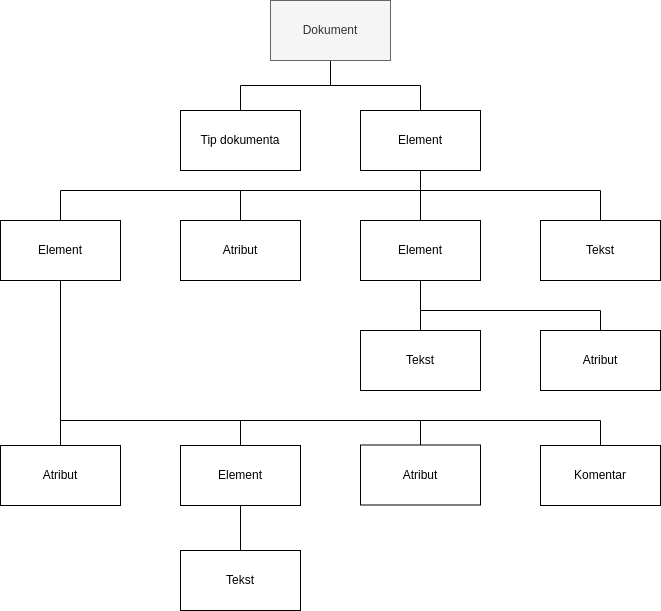
\includegraphics[width=0.9\textwidth]{slike/DOM_stablo.png}
	\caption{DOM stablo}
\end{figure}

\begin{lstlisting}[language=java, caption={Dohvačanje vrijednosti iz DOM stabla}]
public class DOMPrognoza {

    public String ispisPrognoze() {
        Element korijenskiElement = this.xmlDocument.getDocumentElement();

        Element prognozaDatum = (Element) korijenskiElement.getElementsByTagName("DatumTermin").item(0);
        String datum = prognozaDatum.getElementsByTagName("Datum").item(0).getTextContent();

        ...

        String imeGrada = grad.getElementsByTagName("GradIme").item(0).getTextContent();
        Element podatciElement = (Element) grad.getElementsByTagName("Podatci").item(0);
        double temperatura = Double.parseDouble(podatciElement.getElementsByTagName("Temp").item(0).getTextContent());
        String vrijeme = podatciElement.getElementsByTagName("Vrijeme").item(0).getTextContent();

        ...
    }

    Element pronadiGrad(String imeGrada, Element pocetniElement) throws Exception {
        NodeList gradCvorovi = pocetniElement.getElementsByTagName("Grad");
        int len = gradCvorovi.getLength();
        for (int i = 0; i < len; i++) {
            Node gradCvor = gradCvorovi.item(i);
            if (gradCvor.getNodeType() == Node.ELEMENT_NODE) {
                Element gradElement = (Element) gradCvor;
                if (gradElement.getElementsByTagName("GradIme").item(0).getTextContent().equals(imeGrada)) {
                    return gradElement;
                }
            }
        }
        throw new Exception("Grad nije bio pronađen");
    }
\end{lstlisting}

U isječku se nalazi kod koji iz DOM stabla izvlači potrebne podatke za ispis vremenske
prognoze. Metoda \texttt{ispisPrognoze} počinje s dohvaćanjem korijenskog elementa
iz DOM stabla, korijenski element se dohvaća metodom \texttt{getDocumentElement}.
Slijedeće se iz korijenskog elementa dohvaća datum. To se radi na način da na korijenskom
elementu pretražimo sve elemente koji imaju tag \texttt{DatumTermin}.
Metoda \texttt{getElementsByTagName} vraća listu elemenata s određenim nazivom. Kako
smo sigurni da nema više od jednog elementa koristi se metoda \texttt{item(0)}
da se izvadi prvi element u listi. Na isti način se dobiva sam datum iz DatumTermin,
jedina razlika je što na kraju pozivamo metodu \texttt{getTextContent} koja vraća
datum u tekstualnom obliku. Na sličan način se dobivaju ostali podaci kao što su
\texttt{imeGrada}, \texttt{temperatura}, \texttt{vrijeme}.

Druga metoda koja je prikazana u isječku je \texttt{pronadiGrad}. Metoda prolazi kroz
sve elemente koji imaju tag \texttt{Grad}. Za svaki pregledava ako je taj čvor zapravo
tipa element, ako je taj uvjet zadovoljen pretvara trenutni grad iz tipa \texttt{Node}
u tip \texttt{Element} kako bi bilo moguće pregledati podatke o elementu. Slijedeće
pregledava vrijednost sadržanog elementa i ako je vrijednost jednaka ulaznom argumentu
\texttt{imeGrada} metoda vraća pronađeni element.

\section{JAXB}
JAXB (Java Architecture for XML Binding) pruža API za jednostavno pretvaranje objekata
u XML i iz XML-a u objekte. JAXB je vrlo jednostavan za koristiti i zahtjeva najmanje
pisanja koda. Funkcionira kroz korištenje anotacija na postoječim objektima. Anotacijama
se definiraju koji dijelovi objekta spadaju u XML dokument, koji dijelovi su elementi,
koji dio je korijenski element, koje dijelove treba preskočiti jer nisu dio XML kojega
generiramo ili učitavamo. Za definiranje korijenskog elementa na klasu se postavlja
anotacija \texttt{$@$XmlRootElement}, sami elementi se definiraju postavljanjem anotacije
\texttt{$@$XmlElement} na članove klase, atributi se definiraju anotacijom
\texttt{$@$XmlAttribute}. Po potrebi se mogu dodavati anotacija \texttt{$@$XmlTransient}
koja označava da se član klase ne uključuje u Xml dokument ili \texttt{$@$XmlElementWrapper}
u slučaju kad trebamo definirati da će sljedeći element biti sadržan u drugom elementu.

\begin{lstlisting}[language=java, caption={Primjer JAXB anotacija na klasama}]
@XmlRootElement(name = "AgroMeteoroloskiPodaci")
public class MeteoroloskiPodaciTjedanDana {
    @XmlElement(name = "Naslov")
    public String naslov;

    @XmlElementWrapper(name = "Podaci")
    @XmlElement(name = "Grad")
    public ArrayList<Grad> podaci;
}

class Grad {
    @XmlElement(name = "GradIme")
    String gradIme;

    @XmlElement(name = "Tmax")
    String tMax;

    ...

    @XmlElement(name = "Sunce")
    String sunce;

    ...
}
\end{lstlisting}

Isječak prikazuje sav kod koji je potreban za parsiranje ili kreiranje XML dokumenta iz
objekta \texttt{MeteoroloskiPodaciTjedanDana}. Za JAXB dovoljno je postaviti anotacije
i odmah imamo mogućnos rada s XML-om.

\begin{lstlisting}[language=java, caption={Pretvaranje XML dokumenta u Java objekte korištenjem JAXB}]
JAXBContext jaxbContext = JAXBContext.newInstance(MeteoroloskiPodaciTjedanDana.class);
Unmarshaller unmarshaller = jaxbContext.createUnmarshaller();
MeteoroloskiPodaciTjedanDana meteoroloskiPodaci = (MeteoroloskiPodaciTjedanDana) unmarshaller.unmarshal(DemoDatoteke.demoSedmodnevniPodaciXML());
\end{lstlisting}

Kako bi pretvorili XML dokument u java objekt JAXBContext-u se pridaje klasa izlaznih
podataka, kreira se objekt Unmarshaller koji kod korištenja metode \texttt{unmarshal}
prima XML datoteku i direktno je parsira i mapira u zadani objekt.
Suprotno se može postići korištenjem Marshallera koji pretvara postojeći objekt u XML.

\chapter{Zaključak}
Raditi s XML-om u javi je vrlo jednostavno. Postoji veliki broj dostupnih knjižnica koje
omogućuju brz i lagan rad. Ovisno o potrebama moguće je koristiti različite parsere koji
nude različite performanse, načine manipulacijom podataka. Primjena XSD-a prije samog
parsiranja nam garantira da dokument koji se parsira uvijek ima elemente koje očekujemo
u programu te omogućava lakši rad s XML-om i spriječava stvaranje bugova. U projektu nije
obrađen XPath koji omogućuje navigaciju kroz DOM stablo za lakše dohvaćanje podataka
iz stabla, no isto se često koristi u programima.


\printbibliography[title=Popis literature]
\addcontentsline{toc}{chapter}{Popis literature}

\listoffigures
\addcontentsline{toc}{chapter}{Popis slika}

\end{document}
